%@@@@@@@@@@@@@@@@@@@@@@@@@@@@@@@@@@@@@@@@@@@@@@@@@@
\chapter{RVQ in computer vision (tracking)}
\label{chap_RVQ_STT}	
%@@@@@@@@@@@@@@@@@@@@@@@@@@@@@@@@@@@@@@@@@@@@@@@@@@
In this chapter, we build on the theoretical and experimental knowledge that has been explained in the previous chapters.  In the introductory first chapter, we looked at various forms of object representation.  In this chapter, we explain in detail the object representation used in this work.  The second chapter looks at the theoretical aspects of RVQ.  We use the knowledge and notation introduced there and explain how RVQ is used in tracking.  The third chapter begins with the usage of RVQ for recognition on images and transitions to the usage of RVQ for recognition in image sequences.  We take this a step forward and explain how RVQ is used in tracking on image sequences.  The fourth chapter discusses tracking methods used in the literature.  Some standard approaches, including filtering methods and some relatively newer subspace methods were discussed.  We combine these approaches in a manner similar to existing PCA tracking approaches in the literature and extend this work to RVQ and TSVQ tracking.  This is significant since PCA is commonly used in the Pattern Recognition, Machine Learning and Computer Vision communities.  RVQ and TSVQ however are not commonly used in these communities.  On the other hand, two-stage RVQ and multi-stage TSVQ are commonly used in the Signal Processing and Information Theory communities.  By using more-than-two-stage RVQ in visual tracking, we hope that our work will extend and bring together knowledge from different fields and allow researchers to build on the results we present in this chapter, and the conclusions we arrive to in the next.

\begin{table}[t]
\centering
\begin{tabular}{| l | c | c | p{2.5in} |}
\hline
Transformation & DoF & Matrix & Distortion\\ \hline 
& & & \\ Projective & 8 & $\ProjMatrix$ & any arbitrary quadrilateral as long as no three points are collinear\\  & & & \\ \hline
& & & \\ Affine & 6 & $\AffMatrix$ & rotation and non-isotropic scaling\\  & & & \\ \hline
& & & \\ Similarity & 5 & $\SimMatrix$ & scaling and rigid motion\\  & & & \\ \hline
& & & \\ Euclidean & 4 & $\EucMatrix$ & rigid motion (rotation, translation) \\  & & & \\ \hline
\end{tabular}\
\caption{2D transformations}
\label{table:2Dtransformations}
\end{table}

Before continuing, we present a very high level approach taken to tracking in this chapter.  This is exactly the same approach used in Ross et. al. \cite{2008_JNL_subspaceTRK_Ross}.  As a matter of fact, we use the excellent software they have provided on their website \cite{2008_SFT_Ross} and build on it.  The advantage of using existing software is that it is open to scrutiny, avoids duplication of work, avoids implementation mistakes, allows researchers to more readily build on existing work and allows for direct comparisons.  In this spirit, we make our own software available for download at \url{http://users.ece.gatech.edu/~msalman} and also present it in Appendix~\ref{App:software}.  The only code not available for download is the RVQ codebook generation process.  This is a patented technology.  The binaries of this code were provided for this project by the inventor, Dr Christopher Barnes in the Georgia Institute of Technology.

The tracking process in this work comprises the following steps:

\begin{enumerate}
\item \underline{One-time initialization}.  The target is identified in the first frame by drawing a bounding box around it.  The box is allowed to be affinely deformed as discussed later in this chapter.  Template matching then allows a certain number of frames to be designated as initial training frames.  Currently this value is set to $N_B=5$. 

\item \underline{Run-time training}.  After every $N_B$ frames, images in the training buffer are used to train separate models for iPCA, bPCA, RVQ and TSVQ.  The training buffer is composed of the last $N_w$ images.  In this work, experiments are carried out with $N_w=2, 4, 8, 16, 32, 64, 128$ and $\infty$.  Note that this value is different from $N_B$.
  
\item \underline{Run-time testing}.  Every frame after the one-time initialization is tested against the iPCA, bPCA, RVQ and TSVQ models and results are compared.  The Condensation algorithm~\cite{1998_JNL_Condensation_IsardBlake} is used for temporal and spatial integration of observation and state information.  Spatial processing includes generating several candidate window chips (snippets) and picking the one that gives least mean squared reconstruction error.  Temporal processing includes carrying over the posterior density from a frame as the prior density for the next frame.  The snippet that gives the least squared error is retained and added to the pool of training images in FIFO (first-in first-out) fashion, i.e. a moving window of $N_w$ training images is maintained.
\end{enumerate}

In order to accomplish this tracking process, we create the following five models:

\begin{enumerate}
\item \underline{Representation model}.  This model deals with target representation, as shown in Figure~\ref{fig:TRK_objectRepresentations}.  In this work, we represent the target with a bounding quadrilateral that is allowed to undergo affine deformations.
\item \underline{Appearance model}.  Four models are used to model target appearance, two forms of PCA, RVQ and TSVQ.
\item \underline{Motion model}.  The target motion is assumed to be Brownian to deal with arbitrary target and camera motion.
\item \underline{Observation model}.  The observation model ties the observations with the expected state.  We use target reconstruction mean squared error as the metric to score the observations in every frame.
\item \underline{Inference model}.  This model ties in multiple possible spatial observations in a temporal framework to enable sequential inference through the tracking process.
\end{enumerate}

Each of these five models is discussed in more detail in the following five sections.  As a result of this modeling framework, we are able to handle the following scenarios:

\begin{itemize}
\item Representation model related
\begin{enumerate}
\item Target scale changes
\item Target orientation changes
\end{enumerate}
\item Motion model related
\begin{enumerate}\setcounter{enumi}{2}
\item Arbitrary camera motion
\item Arbitary target motion
\end{enumerate}
\item Appearance model related
\begin{enumerate}\setcounter{enumi}{4}
\item Target pose changes
\item Lighting changes
\item Structured noise
\item Temporary occlusions
\end{enumerate}
\end{itemize}


%\begin{itemize}
%\item \underline{Temporary occlusions}.  The occlusions are temporary, on the order of about 10 frames.
%\end{itemize}
%\begin{itemize}
%\item \underline{Perspective changes handled effectively with affine deformation}.  An affine transform in a tracking scenario can deal effectively with a large variety of target deformations, including some perspective effects.  We therefore choose the affine transform in favor of the less restrictive projective transform which can handle severe perspective effects.  A comparison of some 2D geometric transformations is given in Table~\ref{table:2Dtransformations}.
%\end{itemize}

At every frame, we try to estimate a state vector $\mathbf{X}$ in $R^6$.  Two components of this vector, the target coordinates are related to the motion model and the remaining four are related to the affine deformation allowed by the representation model.  To keep our models as general as possible, all 6 components of the state are modeled as Gaussian random variables but with known variance.  However, in order to simplify sampling from the joint density, it is possible to use certain relaxation criteria such as Markovian dependence, or complete independence.  We choose the latter to make the sampling process in the inference model somewhat more straightforward.

Our motion model then consists of 6 uncorrelated gaussian densities. 
The target motion is therefore represented not in analytic form but as a 6x6 diagonal covariance matrix $\Sigma_X$ centered at the target position $\mathbf{X}_{t-1}$ in the previous frame.  The elements on the diagonal represent variances of affine parameters, $\sigma_x^2, \sigma_y^2, \sigma_\theta^2, \sigma_s^2, \sigma_\alpha^2, \sigma_\phi^2$.   


Several Gaussian distributions are used to handle these changes.  One distribution each is used to handle arbitrary translation in the horizontal direction, vertical direction, scale, rotation.  At every time step, predicted values are sampled from these distributions.  Each predicted value is warped to a standard window size and tested against the existing model.  The predicted value closest to the current model is selected as the next estimate and is used to update the model.  In PCA, the model is the eigenvectors, in RVQ, it's the stage codevectors and in TSVQ, it's the terminal codevectors.  

In this work, we model the object motion by an affine image warp.  The state at time $t$ consists of 6 affine transformation parameters: $x_t,  y_t, \theta_t, s_t, \alpha_t$, and $\phi_t$.


We now discuss each of these tracking components one by one.

%#############################
\section{Representation model}
\label{Sec:Representation_model}
%#############################
In this section, we discuss the representation model.  We refer back to Figure~\ref{fig:TRK_objectRepresentations} in the introductory chapter that shows different target representations.  



Table \ref{table:2Dtransformations} shows different kinds of 2D linear transformations.  Every transformation generalizes the transformation below it in the table.  In this work, we use the 2D affine transform since it is flexible enough to account for most distortions in real images.  However, it cannot handle perspective effects, for which a projective transformation is required. The affine transform is given by,

\begin{equation}
\begin{array}{cccc}
\mathbf{\acute{x}} &=& \mathbf{A}\mathbf{x} + \mathbf{t}\\
&=&\mathbf{H}_A \mathbf{x}\\
&=& \left[\begin{array}{cccc}\mathbf{A} & \mathbf{t}\\\mathbf{0}^T & 1\end{array}\right] \mathbf{x}\\
\left[\begin{array}{l}\acute{x}\\\acute{y}\\1\end{array}\right]   &=& \AffMatrix \left[\begin{array}{l}x\\y\\1\end{array}\right]
\end{array}
\end{equation}

$t_x$ and $t_y$ are translations in the $x$ and $y$ directions respectively.  Including these 2 parameters in $\mathbf{H}_A$ allows the affine transformation to be expressed as a single matrix multiply.  

The affine matrix $\mathbf{A}$ can always be decomposed using the SVD decomposition as the product of orthogonal matrices $\mathbf{U}$ and $\mathbf{V}$ and a diagonal matrix $\mathbf{S}$, \cite{2004_BOOK_CG_Hartley}:

\begin{equation}
\begin{array}{llllllll}
\mathbf{A} &= \left[\begin{array}{lll}a_{11} & a_{12} \\ a_{21} & a_{22}\\ \end{array}\right] \\
&=\mathbf{U}{\color{blue}\mathbf{S}}\mathbf{V}^t \\
&={\color{red}(\mathbf{U}\mathbf{V}^t)}\mathbf{V}{\color{blue}\mathbf{S}}\mathbf{V}^t\\
&={\color{red}\mathbf{R}(\theta)}\mathbf{R}(-\phi){\color{blue}\mathbf{S}}\mathbf{R} (\phi)\\
&={\color{red}\RotMatrixTheta}\RotMatrixminusPhi{\color{blue}\EigenvalueMatrix}\RotMatrixPhi\\\\
\end{array}
\label{Eq:AffineDecomposition}
\end{equation}

The affine matrix $\mathbf{A}$ can therefore be viewed as a succession of the following 4 steps:

\begin{enumerate} 
\item Rotation by angle $\phi$ 
\item This rotation is followed by a scaling of $\lambda_1$ and $\lambda_2$ in the rotated $x$ and $y$ directions
\item A rotation by angle -$\phi$ which brings the scaled object back to its original orientation
\item A rotation by angle $\theta$
\end{enumerate}

We now discuss how to go from affine parameters to affine matrix.  For a given tracking scenario, the initial target planar bounding region is more intuitively expressed in terms of the affine parameters $\theta, \phi, \lambda_1, \lambda_2$ than in terms of the affine matrix $\mathbf{A}$.  However, the actual affine warp is more easily carried out using matrix multiplication.  Therefore, computing $\mathbf{A}$ explicitly is often required and can be done by substituting the affine parameters into Equation \ref{Eq:AffineDecomposition} to get,

\begin{equation}
\mathbf{A} = \bigMatrix
\end{equation}
where,

\begin{equation*}
\begin{array}{llll}
\mathrm{ccc} &= \cos(\theta) \cos(\phi) \cos(\phi), & \mathrm{ccs} &= \cos(\theta) \cos(\phi) \sin(\phi)\\
\mathrm{css} &= \cos(\theta) \sin(\phi) \sin(\phi), & \mathrm{scc} &= \sin(\theta) \cos(\phi) \cos(\phi)\\
\mathrm{scs} &= \sin(\theta) \cos(\phi) \sin(\phi), & \mathrm{sss} &= \sin(\theta) \sin(\phi) \sin(\phi)\\
a   &=  \mathrm{css} - \mathrm{scs}, & b   &=  \mathrm{ccc} + \mathrm{scs}\\
c   &= \mathrm{ccs} + \mathrm{sss}, & d   &=  \mathrm{ccs} - \mathrm{scc}\\
s 			    &= \lambda_1, & r 			    &= \frac{\lambda_2}{\lambda_1}\\
\end{array}
\end{equation*}


Here we discuss how to go from affine matrix to affine parameters.  It is possible to recover the affine parameters from the affine matrix using Equation \ref{Eq:AffineDecomposition} again.  $\theta$  can be computed as follows,  

\begin{equation}
\begin{array}{lllllll}
\mathbf{R}(\theta) &= \RotMatrixTheta \\
&= \mathbf{U}\mathbf{V}^T \\
&= \left[\begin{array}{llll}\mathbf{U}(1,1) & \mathbf{U}(1,2)\\\mathbf{U}(2,1) & \mathbf{U}(2,2)\end{array}\right]\left[\begin{array}{llll}\mathbf{V}(1,1) & \mathbf{V}(2,1)\\\mathbf{V}(1,2) & \mathbf{V}(2,2)\end{array}\right] \\
\Rightarrow \theta &= \tan^{-1}\frac{\mathbf{U}(2,1)\mathbf{V}(1,1) + \mathbf{U}(2,2)\mathbf{V}(1,2)}{\mathbf{U}(1,1)\mathbf{V}(1,1) + \mathbf{U}(1,2)\mathbf{V}(1,2)}
\end{array}
\end{equation}

								\begin{figure}[t]
								\centering
								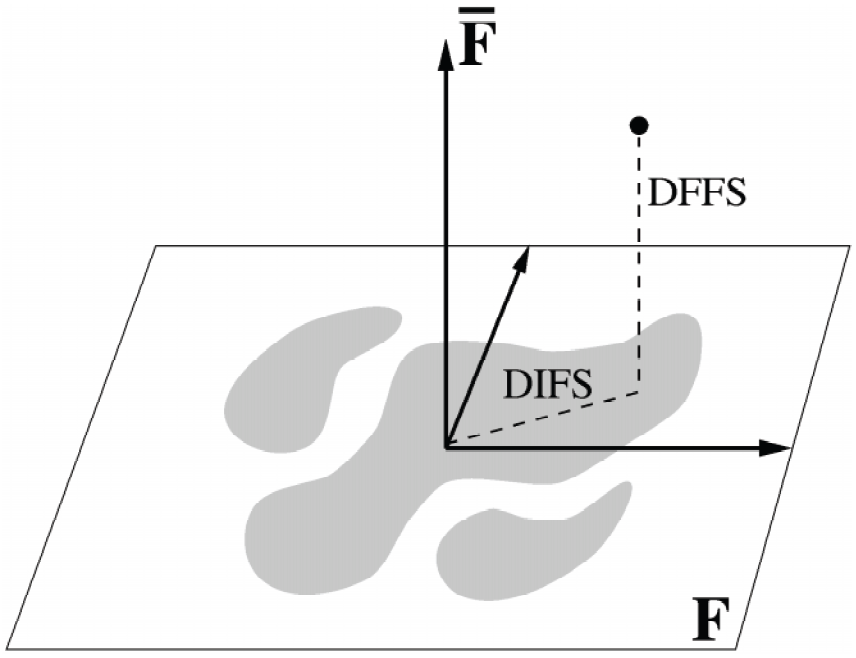
\includegraphics[width=0.5\textwidth]{figs/1998_JNL_ProbVisLearning_Moghaddam_fig3.png}
								\caption{Graphical illustration of DFFS (distance-from-feature-space) and DIFS (distance-in-feature-space).  The feature space is $\mathbf{F}$ while the subspace orthogonal to the feature space is $\bar{\mathbf{F}}$.  DFFS is the signal residual error and DIFS is the $\mathbf{F}$-space likelihood \cite{1997_JNL_EigenTRK_Moghaddam}.}
								\label{fig:1997_JNL_DIFSDFFS_Moghaddam}
								\end{figure}



$\phi$ is computed as follows,

%%%CAUTION: RECONCILE THIS WITH CODE%%%
\begin{equation*}
\phi = \tan^{-1}\frac{\mathbf{V}(2,1)}{\mathbf{V}(1,1)}
\end{equation*}

$s$ and $r$ are computed as follows,

\begin{equation}
\begin{array}{llll}
s &= \lambda_1 &=  \mathbf{S}(1,1)\\
r &= \frac{\lambda_2}{\lambda_1} &= \frac{\mathbf{S}(2,2)}{\mathbf{S}(1,1)}
\end{array}
\end{equation}


A target is initially specified using a rotated bounding box which requires 5 parameters for complete specification:

\begin{enumerate}
\item $x_c$, bounding box center x coordinate
\item $y_c$, bounding box center y coordinate
\item $w$, width of bounding box
\item $h$, height of bounding box
\item $\theta$, rotation angle of bounding box in radians.  Counter-clockwise rotations of the bounding box are taken as negative angles.  
\end{enumerate}

%\item \underline{Target scale and orientation changes}.  Since we choose to model the deformations in the target bounding quadrilateral with an affine transform, we can handle target scale and orientation changes.  
%\end{enumerate}
%Another aspect is that we allow for pose and scale changesthe target bounding quadrilateral to undergo affine deformation.  The state vector $\mathbf{X}$  instead of constituting the commonly used $(x,y)$ coordinates of the target now constitutes 


%########################
\section{Motion model}
%########################
The motion model is a mathematical representation of the real or expected motion of the target of interest.  Since tracking is in general an ill-posed problem, it is common to make assumptions about the motion to simplify motion modeling.  Common assumptions such as stationary camera, coherent motion etc. are discussed in Chapter~\ref{chap_Tracking_methods}.

In this work, we make two assumptions about the target motion:

\begin{itemize}
\item \underline{Coherent motion}.  We assume that each part of the target moves together.  The target can deform and warp but it does not break up into individual parts.
\item \underline{Can be modeled with a gaussian distribution with fixed variance}.  We assume that the motion is brownian and can be modeled with a gaussian distrubution with a fixed variance.  
\end{itemize}

An advantage of not having an explicit motion model is that arbitrary camera and target motion are allowed.  A disadvantage of this approach in the context of the particle filter is that particles need to be evaluated all around the current target position, rather than only around the projected target position.  We are therefore unable to take advantage of the reduced spatial search-space that comes with a deterministic motion model.  

Two of the six components of the state vector $\mathbf{X}$ deal with the motion model.  These are the $x$ and $y$ coordinates of the target.  These are modeled as independent gaussian random variables with fixed variance $\sigma_x^2, \sigma_y^2$,

\begin{align*}
p(x_t|x_{t-1}) &= \mathcal{N}(x_{t-1}, \sigma_x^2) \\
p(y_t|y_{t-1}) &= \mathcal{N}(y_{t-1}, \sigma_y^2) \\
\end{align*}

%########################
\section{Observation model}
%########################
An observation model $p(z_t|x_t)$ relates the state $x_t$ at time $t$ to the observation $z_t$ at time $t$.  Unfortunately, it is not possible to estimate it from the data and so reasonable assumptions must be made.  The observations are assumed to be independent of each other as well as of the dynamical process \cite{1998_JNL_Condensation_IsardBlake}. 

In this work, for PCA, the observation model assumes that the candidate window chips (snippets) in the image that can contain the target were generated from a subspace of the target $\mathbf{U}$ centered at $\mathbf{\mu}$.  The distance metric used to score each candidate window is explained in Section~\ref{Sec:Chap5_PCA}.  For RVQ and TSVQ, the observation model assumes that the candidate snippets were generated from the RVQ and TSVQ codebooks respectively.  The distance metric used to score snippets is based on the mean squared reconstruction error.  For RVQ, an additional constraint is monotonic SNR increase in the DSSA (direct sum successive approximation) reconstruction.  In other words, not all RVQ stages have to be used to reconstruct the target.  The reconstruction must stop if the stage code-vector at the next additive stage does not result in SNR increase.


%\begin{figure}
%\centering
%\includegraphics[width=0.75\textwidth]{figs/1998_JNL_Condensation_Isard_fig7.png}
%\caption{}
%\label{fig:1998_JNL_Condensation_Isard_fig7}
%\end{figure}


%#######################		
\section{Appearance model}
\label{Sec:RVQ_trk_appearance_model}
%#######################
The appearance model of a target is an abstraction for the intensity values of its pixels.  Common appearance models include just the raw values of the pixel intensities, intensity distributions, pixel intensity centroids, etc.  In this work, we choose three appearance models based on PCA, RVQ and TSVQ.  In each case, the appearance model is updated every $N_B$ frames, chosen to be 5 in this work for accurate comparison with~\cite{2008_JNL_subspaceTRK_Ross}.    This updating allows the tracker to deal with changing target pose, lighting changes, structured noise and temporary occlusions.   





We now look at each of these methods in turn.

%======================
\subsection{PCA}
\label{Sec:Chap5_PCA}
%======================

In this work, for PCA, it is assumed that an image $\mathbf{X}$ in $R^D$ is probabilistically generated from a subspace $\mathbf{U}$ spanned by earlier observed images.  The covariance matrix $\Sigma$ of the input training images can be written as follows,  

\begin{equation}
\Sigma = \mathbf{U}\mathbf{\Lambda} \mathbf{V}^T
\end{equation}

Here $\mathbf{\Lambda}$ is the matrix of eigenvalues.  The distribution is assumed to be Gaussian centered at $\mathbf{\mu}$.  The probability of an image being generated under this distribution is inversely proportional to its distance from $\mathbf{\mu}$.  This distance can be decomposed into two parts:

\begin{enumerate}
\item DFFS (distance-from-feature-space):  In a partial KL expansion using $Q$ eigenvectors, the space spanned by these $Q$ eigenvectors is given by $\mathbf{F}$ and the signal residual $\epsilon^2$ is given by

\begin{equation}
\epsilon^2 = \Vert \tilde{\mathbf{X}} \Vert^2 - \sum\limits_{i=1}^M \mathbf{u}_i^2 = \sum\limits_{i=M+1}^D \mathbf{u}_i^2
\end{equation}

where $\mathbf{u}_i$ are the eigenvectors of $\Sigma\Sigma^T$ and $\tilde{\mathbf{X}}$ is the mean removed input image.  This signal residual is referred to as DFFS.
\item DIFS (distance-in-feature-space):  This is the component of $\mathbf{X}$ which lies in the feature space $\mathbf{F}$.  
\end{enumerate}

DIFS and DFFS are illustrated graphically in Figure~\ref{fig:1997_JNL_DIFSDFFS_Moghaddam}.  

%This leads the likelihood function to be a function of two distributions,
%
%\begin{equation}
%p(\mathbf{I}|\mathbf{X}) =  \mathcal{N}()
%\end{equation}
%
%\begin{equation}
%p(I_t|X_t) = \mathcal{N}
%\end{equation}

%======================
\subsection{RVQ}
\label{Sec:Chap5_RVQ}
%======================
For RVQ, the appearance model is exactly the same as that used in Chapter~\ref{chap_RVQ_CV_recog}.  The only difference is that the codebooks are now dynamic and updated every $N_B=5$ frames. 

%======================
\subsection{TSVQ}
\label{Sec:Chap5_TSVQ}
%======================
The Tree Structured Vector Quantizer (TSVQ) has received a lot of attention in the literature~\cite{1991_BOOK_VQ_GershoGray}.  The reason is that the codebook produced by a TSVQ approximates the codebook produced by an Exhaustive Search Vector (ESVQ) but the run-time computational cost is logarithmic in the number of code-vectors.  The storage requirements however are greater.  A comparison of ESVQ, TSVQ and RVQ can be seen in Table~\ref{tab:comparison_ESVQ_TSVQ_RVQ}.

In TSVQ design, the first step is to compute the mean of the data.  All the data is mapped to this mean.  The mean is then split off into $M_{TSVQ}$ centroids (code-vectors).  For a binary TSVQ, $M=2$.  The data is mapped to these centroids using the Nearest Neighbor rule.  Each of these $M_{TSVQ}$ parent centroids is then again split into $M_{TSVQ}$ child centroids.  Splitting can be achieved by multiple iterations of the K-means algorithm to get centroids that give low mean squared error.  At every stage of the tree, data belonging to a parent code-vector is mapped to the child code-vectors after the splitting occurs.  Notice that the important code-vectors are the last stage children code-vectors, i.e. the terminal leaves of the tree.  However, during run-time, the parent code-vectors, i.e., the non-terminal nodes of the tree have to be stored in order to be able to traverse the tree to get to the terminal code-vectors.  The process of mapping data at run-time to the terminal code-vectors is quite straightforward.  The data is first mapped to the mean, which is a trivial step, since all data starts at the top of the tree, i.e., the mean.  Each data-point is then mapped to one of the two children nodes at the first stage using the Nearest Neighbor method.  This process continues till a terminal code-vector is reached which is then used as an approximation to the input data-point.

In this work, we use a binary and balanced TSVQ.  In the binary case, the storage requirements are double the storage requirements for an equivalent ESVQ.  However, the run-time savings decrease logarithmically.  For instance, a codebook size of $K=256$ requires 256 matches for ESVQ but only 8 matches for a binary TSVQ.  

During tracking, a TSVQ codebook is designed every $N_B=5$ frames using $N_w$ images in the training buffer.  The particle filter candidate target regions in the current frame are tested against this code-book, i.e., for each candidate region, the terminal code-vector  to the mean squared error between that region and the terminal code-vector in the tree that 

The candidate that gives least mean squared error is chosen as the most likely  to find the terminal code-vector in the TSVQ tree that minimizes mean-squared error.  

%#######################		
\section{Inference model}
%#######################
The inference model in this work is based on a sequential Monte Carlo (SMC) filter, the particle filter.  The particle filter has been discussed in Chapter~\ref{chap_Tracking_methods}.  Almost all particle filters are based on the sequential importance sampling (SIS) algorithm, including the sampling importance resampling (SIR) filter, auxiliary sampling importance resampling (ASIR) filter and the regularized particle filter (RPF).  The basic difference between these algorithms is the choice of \emph{importance sampling density} and/or modification of the resampling step~\cite{2002_JNL_PF_Arulampalam}.  

In this work, we use the basic SIS algorithm.  It is essentially the same as the SIR filter except that there is no resampling step.  However, like the SIR filter, we use the prior density as the importance sampling density.  The weights on the posterior are computed using the appearance model for PCA, RVQ or TSVQ, depending on which of these algorithms is being used.  For RVQ for instance, the mean squared reconstruction error is used for the weighting.

The number of particles used is $N_p=600$.  Each particle represents the point mass density of a vector $\mathbf{X}$ in $R^6$ corresponding to the 6 parameters required for an affine deformation.

\cite{1992_JNL_MCMC_Carlin}
%########################
\section{Results}
%########################
%===========================
\subsection{Detection, static codebooks}
%===========================
								\begin{figure}[t]
								\centering	
								\subfigure[Input image.]{\includegraphics[width=0.75\textwidth]{figs/Exp_GT1_input_RVQ_FN0_snippets.pdf}}
								\subfigure[Reconstruction SNR (scaled between 0 and 255, 2D and 3D plots).]{\includegraphics[width=1.0\textwidth]{figs/Exp_GT1_results_RVQ_corstgidx_noStages.png}}
								\caption{RVQ detections, static codebooks.  Several background pixels are included with the target causing high reconstruction SNR in regions other than the target.}										
								\label{fig:RVQdet_staticCB_oneTarget}				
								\end{figure}


We now turn to the usage of RVQ in visual tracking.  

In Figure~\ref{fig:RVQdet_staticCB_oneTarget}, we pick 23 snippets from different parts of a single target to be tracked and train an 8x4 codebook on it.  Upon reconstruction, we would like high SNR to be achieved only in regions occupied by the target.  However, since background pixels from background plants are also included in the training data, high SNR is achieved wherever there are green plants in the entire image.  The target region though has high SNR as expected.  

								\begin{figure}[t]
								\centering	
								\subfigure[Training image.]{\includegraphics[width=0.65\textwidth]{figs/Exp_GT1_input_RVQ_multi_target_snippets.pdf}}
%								\subfigure[Training image, SNR.]{\includegraphics[width=0.3\textwidth]{figs/Exp_GT1_results_RVQ_FN0_cor2D.pdf}}
%								\subfigure[Test image, SNR.]{\includegraphics[width=0.3\textwidth]{figs/Exp_GT1_results_RVQ_FN2_cor2D.pdf}}\\
								\subfigure[8x4 codebook]{\includegraphics[width=0.32\textwidth]{figs/Exp_GT1_results_RVQ_codebooks.png}}\\
								\subfigure[Training image, SNR.]{\includegraphics[width=0.23\textwidth]{figs/Exp_GT1_results_RVQ_FN0_cor3D.pdf}}
								\subfigure[Test image, SNR.]{\includegraphics[width=0.23\textwidth]{figs/Exp_GT1_results_RVQ_FN2_cor3D.pdf}}
								\subfigure[Training image, stages.]{\includegraphics[width=0.23\textwidth]{figs/Exp_GT1_results_RVQ_FN0_stg.pdf}}
								\subfigure[Test image, stages.]{\includegraphics[width=0.23\textwidth]{figs/Exp_GT1_results_RVQ_FN2_stg.pdf}}
%								\subfigure[Training image, detection.]{\includegraphics[width=0.3\textwidth]{figs/Exp_GT1_results_RVQ_FN0_stgsnr.pdf}}
%								\subfigure[Test image, detection.]{\includegraphics[width=0.3\textwidth]{figs/Exp_GT1_results_RVQ_FN2_stgsnr.pdf}}
								\caption{RVQ detections, static codebooks.  Background pixels are minimized resulting in better localization.}										
								\label{RVQdet_staticCB_manyTargets}				
								\end{figure}


In Figure~\ref{RVQdet_staticCB_manyTargets}, we attempt to minimize inclusion of background pixels.  Nine snippets per target for six different targets are picked and used to train an 8x4 codebook.  The codebook shows that all four codevectors in the top-level stage represent targets with different textures.  Since target 1 and target 4 in Figure~\ref{RVQdet_staticCB_manyTargets} are wearing shirts with similar hue and texture, they share a common top level code-vector.   During testing phase, it can be seen that reconstruction SNR in the sky region has been minimized.  However, the grass region has high SNR since the texture of one of the targets resembles the grass.  Overall localization has nevertheless been improved in both the training and test images.  Notice that the sky in the top of the image and large grass patch in the lower part of the image need less stages for reconstruction under the monotonic SNR increase condition, i.e., the reconstruction process is terminated at a stage if the next additive stage does not result in an SNR increase.  
								\begin{figure}[t]
								\centering	
								\subfigure[Input image.]{\includegraphics[width=0.3\textwidth]{figs/RVQ_trk_dynamicCB_detections_input.png}}
								\subfigure[8x4 codebook trained from previous 4 images.]{\includegraphics[width=0.3\textwidth]{figs/RVQ_trk_dynamicCB_detections_CB.png}}
								\subfigure[Reconstruction SNR.]{\includegraphics[width=0.4\textwidth]{figs/RVQ_trk_dynamicCB_detections_SNR.png}}
								\subfigure[Reconstruction stages.]{\includegraphics[width=0.3\textwidth]{figs/RVQ_trk_dynamicCB_detections_stg.png}}
								\subfigure[Top 7 detections.]{\includegraphics[width=0.3\textwidth]{figs/RVQ_trk_dynamicCB_detections_output.png}}
								\caption{RVQ detections, dynamic codebooks, PETS2001 dataset, frame 624.  The top 7 detections in the entire image fall on the target.  For the codebook display above, the stages increase horizontally (displayed this way to save space).}										
								\label{RVQtrk_dynamicCB_manyTargets}				
								\end{figure}
This is because smooth regions in the image such as grass and sky use few stages since they are explained by the smoother stage code-vectors in the top few stages.  Here the test image is separated from the training image by only 2 frames.  Codebook retraining may be required if the test image is separated by more frames from the test image.  In general, the retraining frequency is determined by how quickly the target changes appearance and will vary from dataset to dataset.

So far, we've discussed RVQ detections using static codebooks.  The following observations were made in these experiements:

\begin{enumerate}
\item \underline{Background pixels.}  Training snippets should be carefully picked to minimize inclusion of background pixels.
\item \underline{Smooth regions in image.}  Smooth regions in the image can have high reconstruction SNR even if the number of reconstruction stages is low.
\item \underline{Non-smooth regions in target.}   Non-smooth regions of the target will have high SNR and high number of reconstruction stages.
\item \underline{Max SNR does not always coincide with max stages}.  The region with the highest SNR in the image does not necessarily have the maximum number of stages.  
\end{enumerate}

								\begin{figure}[t]
								\centering
								\includegraphics[width=1.0\textwidth]{figs/results_RVQtrk_Dudek_RVQcomparison_00028.png}
								\caption{RVQ comparison.  The criterion for "best" snippet in RVQ1 is maximum reconstruction SNR.  In RVQ2, the criterion is maximum reconstruction SNR given maximum number of reconstruction stages.}
								\label{fig:results_RVQtrk_Dudek_RVQcomparison_00028}
								\end{figure}
%===========================
\subsection{Detection, dynamic codebooks}
%===========================
We now turn to exploring dynamic codebooks.  Before beginning the process of tracking, we first try to explore how good RVQ detections are with dynamic codebooks.  If the detections are good, we can expect good tracking.  However, in order to use dynamic codebooks, either tracking has to be carried out so that $N_w$ snippets of the target can be collected for training or ground truth information must be available.  In order to use an incremental methodology, we use the latter approach.  We use ground truth information to train the dynamic RVQ codebooks every 4 frames.  However, the detection process itself does not make use of any ground truth information.  Figure~\ref{RVQtrk_dynamicCB_manyTargets} shows an example frame using this approach.  The input image size is 640x480 pixels.  The snippet size is 41x11 snippets.  At every frame, a total of 620x440=272,800 unique possible rectangular snippets that can be generated in the image are reconstructed using the current codebook.  Of all reconstructions that use the full 8 stages, the reconstructed snippet that has the maximum reconstruction SNR is declared a detection.  Of 181 images tested, there is only one incorrect detection.  Furthermore, it happens when the target emerges from behind an occlusion.  This is 99.45\% correct detection rate.  With these encouraging detection results with dynamic codebooks, we now move to tracking with dynamic codebooks.

								\begin{figure}[t]
								\centering	
								\subfigure[Frame 28.]{\includegraphics[width=0.35\textwidth]{figs/dataset_Dudek_00028.pdf}}
								\subfigure[RVQ1 recon.]{\includegraphics[width=0.22\textwidth]{figs/results_RVQtrk_Dudek_RVQcomparison_small_00028_RVQ1.png}}
								\subfigure[RVQ2 recon.]{\includegraphics[width=0.22\textwidth]{figs/results_RVQtrk_Dudek_RVQcomparison_small_00028_RVQ2.png}}
								\subfigure[Frame 53.]{\includegraphics[width=0.35\textwidth]{figs/dataset_Dudek_00053.pdf}}
								\subfigure[RVQ1 recon.]{\includegraphics[width=0.22\textwidth]{figs/results_RVQtrk_Dudek_RVQcomparison_small_00053_RVQ1.png}}
								\subfigure[RVQ2 recon.]{\includegraphics[width=0.22\textwidth]{figs/results_RVQtrk_Dudek_RVQcomparison_small_00053_RVQ2.png}}
								\subfigure[Frame 74.]{\includegraphics[width=0.35\textwidth]{figs/dataset_Dudek_00074.pdf}}
								\subfigure[RVQ1 recon.]{\includegraphics[width=0.22\textwidth]{figs/results_RVQtrk_Dudek_RVQcomparison_small_00074_RVQ1.png}}
								\subfigure[RVQ2 recon.]{\includegraphics[width=0.22\textwidth]{figs/results_RVQtrk_Dudek_RVQcomparison_small_00074_RVQ2.png}}
								\caption{The reconstruction images for RVQ2 seem to have 2 superimposed images.}										
								\label{fig:results_RVQtrk_comparison_RVQ1_RVQ2}				
								\end{figure}

%===========================
\subsection{Tracking, dynamic codebooks}
%===========================
Now, after examining the behavior of RVQ in face recognition, action recognition, static codebook detections and dynamic codebook detections, it is expected that enough understanding has been obtained to try to tackle one of the most challenging problems in computer vision, visual tracking.

The first question that needs to be answered is which of these two criteria should be used to pick the "best" snippet: (a) maximum SNR, or (b) maximum SNR given maximum reconstruction stages.

								\begin{figure}[t]
								\centering
								\includegraphics[width=1.0\textwidth]{figs/results_RVQtrk_Dudek_RVQcomparison_00080.png}
								\caption{Tracking fails for RVQ2.}
								\label{fig:results_RVQtrk_Dudek_RVQcomparison_00080}
								\end{figure}


To test this, we setup our particle filter tracking set-up for two kinds of RVQ that use one of the two above-mentioned criteria.  Sample results are shown in Figures~\ref{fig:results_RVQtrk_Dudek_RVQcomparison_00028} and~\ref{fig:results_RVQtrk_comparison_RVQ1_RVQ2}.  In the top right image in Figure~\ref{fig:results_RVQtrk_Dudek_RVQcomparison_00028}, the plotted line shows number of stages in the RVQ1 codebook $\sigma$-tree.  The dots show the number of stages in the RVQ2 codebook $\sigma$-tree.  For this particular frame, they are equal.  The last image in the second line shows that RVQ1 uses 2 stages while RVQ2 uses 6 stages.  However, the test SNR plot shows that RVQ1 has higher reconstruction SNR, even though it uses less stages.  This shows that using maximum SNR alone seems to be a better criterion than using maximum SNR given maximum number of stages.  The reason is that if reconstruction begins with an incorrect top-stage code-vector, then several stages are needed to correct this initial mistake.  Several residual stages can be used with increasing reconstruction SNR at every stage, but this may not necessarily create an accurate representation of the target.  Indeed, Figure~\ref{fig:results_RVQtrk_comparison_RVQ1_RVQ2} shows three examples of this.  In all three examples, it is clear that RVQ2 begins with an incorrect top-stage code-vector and additional stages are used in an attempt to correct this mistake.  The result is an apparent superposition of two faces.  In detections, the method of picking highest reconstruction SNR given maximum number of stages worked because the result of one detection does not affect later detections.  In the case of tracking, a few mistakes causes the tracking to fail, and indeed, the tracking fails for RVQ2 as shown in Figure~\ref{results_RVQtrk_Dudek_RVQcomparison_00080.png}. 

Another point to be made is that during face recognition in Chapter~\ref{chap_RVQ_CV_recog}, we made use of the Markovian nature of the XDR $T$-tuple.  This was done since the XDRs for a particular class were quite similar.  The reason for this similarity was that the RVQ $\sigma$-tree was designed using images from all classes.  Therefore, members of a particular class were more likely to have a similar entry point into the RVQ $\sigma$-tree.  Similarly, members of a class were more likely to map to certain residual stage code-vectors.  On the other hand, if an RVQ $\sigma$-tree is designed using images from only one class, as is the case here in tracking, then the stage code-vectors at a particular stage are much more likely to change or inter-change making it difficult to establish a Markovian structure on the XDR.  As a result, we conclude that in tracking scenarios where a codebook is trained for one target, the RVQ criterion for "best" snippet is maximum SNR.

Having done this experimentation with RVQ tracking using dynamic codebooks, we now turn to comparing RVQ tracking on a wide variety of datasets.  We use the datasets given in Table~\ref{Tab:datasets_used}.  Notice that these datasets cover a wide variety of situations.





\begin{table}[t]
\footnotesize
\begin{tabular}{c|ccccccccccccccccccc}
\parbox[c]{0.3in}{\center Dataset} 		&\parbox[c]{0.25in}{\center Scenario} 	     &\parbox[c]{0.4in}{\center Time of \\day} 	&\parbox[c]{0.26in}{\center Target of \\interest} 	&\parbox{0.2in}{\center \# of \\targets} &\parbox{0.3in}{\center Rigid \\target} 	&\parbox{0.4in}{\center Lighting change 1-5 \\(5 most severe)}  	&\parbox{0.45in}{\center Structured \\noise} 	&\parbox{0.3in}{\center Camera \\motion} 	&\parbox{0.2in}{\center Pose \\change} 	&\parbox{0.45in}{\center Expression \\change} 	&\parbox{0.3in}{\center Temporary \\occlusion} 	\\\hline
Dudek 			&Indoors 	     &N/A 			&human 				&1 	&no 	&1 	&yes 	&yes 	&yes 	&yes 	&yes 		\\\hline
davidin300 	&Indoors		&N/A			&human				&1 	&no	&2	&yes	&yes	&yes	&yes	&no		\\\hline
sylv				&Indoors		&N/A			&toy					&1	&yes	&4	&no	&yes	&yes	&N/A	&no		\\\hline
trellis70	 		&Outdoors 		&day, dark		&human				&1	&no	&5	&no	&yes	&yes	&yes	&no		\\\hline
fish				&Indoors		&N/A			&object				&1	&yes	&4	&no	&yes	&no	&N/A	&no		\\\hline
car4			&Outdoors 		&day, sunny	&vehicle				&1	&yes	&3	&no	&yes	&yes	&N/A	&no		\\\hline
car11			&Outdoors		&night			&vehicle				&1	&yes	&4	&no	&yes	&yes	&N/A	&no		\\\hline
\end{tabular}
\caption{Datasets used for RVQ tracking.}
\label{Tab:datasets_used}
\end{table}













\begin{figure}
\centering
\includegraphics[width=0.8\textwidth]{figs/results_lostTrk_bPCA_16_Nw_16_FN_100.pdf}
\caption{Exploring tracking drift in 16-eigenvector batch-PCA (bPCA\_16) with 16 image training window ($N_w=16$).  First of three snapshots.  Refer to Figures~\ref{fig:results_lostTrk_bPCA_16_Nw_16_FN_107} and \ref{fig:results_lostTrk_bPCA_16_Nw_16_FN_136} for the next two snapshots.}
\label{fig:results_lostTrk_bPCA_16_Nw_16_FN_100}
\end{figure}

 
\begin{figure}
\centering
\includegraphics[width=0.8\textwidth]{figs/results_lostTrk_bPCA_16_Nw_16_FN_107.pdf}
\caption{Exploring tracking drift in 16-eigenvector batch-PCA (bPCA\_16) with 16 image training window ($N_w=16$).  Second of three snapshots.  Refer to Figures~\ref{fig:results_lostTrk_bPCA_16_Nw_16_FN_100} and \ref{fig:results_lostTrk_bPCA_16_Nw_16_FN_136} for the first and third snapshots.  Notice that RVQ produces the best reconstruction during this temporary but heavy occlusion as the target completely covers his face.}
\label{fig:results_lostTrk_bPCA_16_Nw_16_FN_107}
\end{figure}


\begin{figure}
\centering
\includegraphics[width=0.8\textwidth]{figs/results_lostTrk_bPCA_16_Nw_16_FN_136.pdf}
\caption{Exploring tracking drift in 16-eigenvector batch-PCA (bPCA\_16) with 16 image training window ($N_w=16$).  Last of three snapshots.  Refer to Figures~\ref{fig:results_lostTrk_bPCA_16_Nw_16_FN_100} and \ref{fig:results_lostTrk_bPCA_16_Nw_16_FN_107} for the first two snapshots.}
\label{fig:results_lostTrk_bPCA_16_Nw_16_FN_136}
\end{figure}


In Figure~\ref{fig:results_lostTrk_bPCA_16_Nw_16_FN_100}, the top row shows that the target bounding box tightly encloses the target for iPCA\_16, bPCA\_16, RVQ\_8x2 and TSVQ\_3.  The instantaneous tracking error, instantaneous training error and instantaneous test errors are also in this row.  The second row shows the instantaneous test SNR (dB), average tracking error, average training error and average test error.     The third and fourth rows show image reconstruction and reconstructed error.  The fifth and final row shows the 600 particle-filter candidate affine-parameterized bounding-quadrilaterals.  All metrics are within reasonable limits for all algorithms.  Seven frames later in Figure~\ref{fig:results_lostTrk_bPCA_16_Nw_16_FN_107}, the target is temporarily but heavily occluded.  The tracking and test errors suddenly jump while test SNR drops.  Notice that RVQ produces the most accurate reconstruction.  Figure~\ref{fig:results_lostTrk_bPCA_16_Nw_16_FN_136} shows that about 30 frames later, iPCA, RVQ and TSVQ have all recovered while bPCA has not recovered, and is unable to recover till the end of the sequence.  This is the reason for the high tracking error for $N_w=4$, bPCA\_16 in Figure~\ref{results_errTrk_3_____1___Dudek}. 



								\begin{figure}[t]
								\centering	
								\subfigure[Average tracking error.]{\includegraphics[width=0.3\textwidth]{figs/results_overall_avg_trk_err.pdf}}
								\subfigure[Average training error.]{\includegraphics[width=0.3\textwidth]{figs/results_overall_avg_trg_err.pdf}}
								\subfigure[Average test error.]{\includegraphics[width=0.3\textwidth]{figs/results_overall_avg_tst_err.pdf}}
								\caption{Average error over all sequences and all configurations when track was held.}										
								\label{fig:averages}				
								\end{figure}

								\begin{figure}[t]
								\centering	
								\subfigure[iPCA.]{\includegraphics[width=0.3\textwidth]{figs/overall_iPCAconfigs_trk_err.pdf}}
								\subfigure[bPCA.]{\includegraphics[width=0.3\textwidth]{figs/overall_bPCAconfigs_trk_err.pdf}}\\
								\subfigure[RVQ.]{\includegraphics[width=0.3\textwidth]{figs/overall_RVQconfigs_trk_err.pdf}}
								\subfigure[TSVQ.]{\includegraphics[width=0.3\textwidth]{figs/overall_TSVQconfigs_trk_err.pdf}}
								\caption{Average tracking error over all sequences when track was held.}										
								\label{fig:averages}				
								\end{figure}


								\begin{figure}[t]
								\centering	
								\subfigure[iPCA.]{\includegraphics[width=0.3\textwidth]{figs/overall_iPCAconfigs_trk_hold.pdf}}
								\subfigure[bPCA.]{\includegraphics[width=0.3\textwidth]{figs/overall_bPCAconfigs_trk_hold.pdf}}\\
								\subfigure[RVQ.]{\includegraphics[width=0.3\textwidth]{figs/overall_RVQconfigs_trk_hold.pdf}}
								\subfigure[TSVQ.]{\includegraphics[width=0.3\textwidth]{figs/overall_TSVQconfigs_trk_hold.pdf}}\\
								\subfigure[Overall.]{\includegraphics[width=0.3\textwidth]{figs/results_correct_trk_percent.pdf}}
								\caption{Percentage of times that the algorithms were able to hold track.}										
								\label{fig:averages}				
								\end{figure}









%Figures~\ref{fig:results_errTrk_3_____1___Dudek, fig:results_errTrk_3_____2___davidin300, fig:results_errTrk_3_____3___sylv, fig:results_errTrk_3_____4___trellis70, fig:results_errTrk_3_____5___car4, fig:results_errTrk_3_____6___car11} show tracking results for different configurations of iPCA, bPCA, RVQ and TSVQ over the different datasets described in Table~\ref{Tab:datasets_used}.  The individual results are shown to get a general idea of how the different algorithms performed on the individual datasets.  Whereas it is useful to look at each individually, the non-linear process of tracking, and the non-linear nature of some of the algorithms involved, i.e., RVQ and TSVQ makes it difficult to draw conclusions from any one dataset alone.  Moreover, numerical issues can cause a particular configuration to lose track in rare cases.  An example of this is shown in Figure~\ref{fig:results_errTrk_3_____1___Dudek} for bPCA-128, $N_w=4$ where different versions of Matlab can produce slightly different results, as discussed in online forums, and which causes bPCA to lose track after a target emerges from occlusion.  








%\begin{figure}
%\centering	
%\subfigure[frames 1, 100, 200, 300, 400]{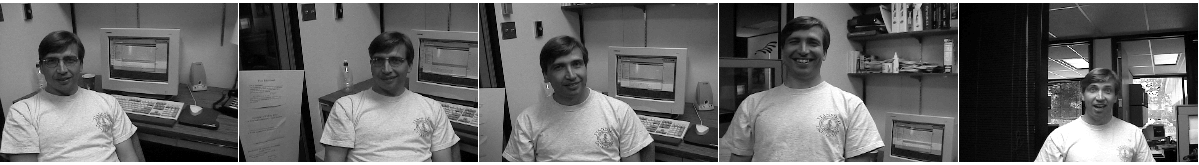
\includegraphics[height=0.1\textheight]{figs/seq_1_Dudek.png}}
%\subfigure[$N_w=2$]{\includegraphics[width=0.3\textwidth]{figs/results_errTrk_3_____1___Dudek___________Nw_0002.pdf}}
%\subfigure[$N_w=4$]{\includegraphics[width=0.3\textwidth]{figs/results_errTrk_3_____1___Dudek___________Nw_0004.pdf}}
%\subfigure[$N_w=8$]{\includegraphics[width=0.3\textwidth]{figs/results_errTrk_3_____1___Dudek___________Nw_0008.pdf}}
%\subfigure[$N_w=16$]{\includegraphics[width=0.3\textwidth]{figs/results_errTrk_3_____1___Dudek___________Nw_0016.pdf}}		
%\subfigure[$N_w=32$]{\includegraphics[width=0.3\textwidth]{figs/results_errTrk_3_____1___Dudek___________Nw_0032.pdf}}
%\subfigure[$N_w=64$]{\includegraphics[width=0.3\textwidth]{figs/results_errTrk_3_____1___Dudek___________Nw_0064.pdf}}
%\subfigure[$N_w=128$]{\includegraphics[width=0.3\textwidth]{figs/results_errTrk_3_____1___Dudek___________Nw_0128.pdf}}
%\subfigure[$N_w=\infty$]{\includegraphics[width=0.3\textwidth]{figs/results_errTrk_3_____1___Dudek___________Nw_10000.pdf}	}
%\caption{Sequence Dudek, tracking error, for a given number of training images ($N_w$), effect of varying algorithm parameters}										
%\label{fig:results_errTrk_3_____Dudek}				
%\end{figure}
%
%
%\begin{figure}
%\centering	
%\subfigure[frames 1, 100, 200, 300, 400]{\includegraphics[height=0.1\textheight]{figs/seq_2_davidin300.png}}
%\subfigure[$N_w=2$]{\includegraphics[width=0.3\textwidth]{figs/results_errTrk_3_____2___davidin300______Nw_0002.pdf}}
%\subfigure[$N_w=4$]{\includegraphics[width=0.3\textwidth]{figs/results_errTrk_3_____2___davidin300______Nw_0004.pdf}}
%\subfigure[$N_w=8$]{\includegraphics[width=0.3\textwidth]{figs/results_errTrk_3_____2___davidin300______Nw_0008.pdf}}
%\subfigure[$N_w=16$]{\includegraphics[width=0.3\textwidth]{figs/results_errTrk_3_____2___davidin300______Nw_0016.pdf}}		
%\subfigure[$N_w=32$]{\includegraphics[width=0.3\textwidth]{figs/results_errTrk_3_____2___davidin300______Nw_0032.pdf}}
%\subfigure[$N_w=64$]{\includegraphics[width=0.3\textwidth]{figs/results_errTrk_3_____2___davidin300______Nw_0064.pdf}}
%\subfigure[$N_w=128$]{\includegraphics[width=0.3\textwidth]{figs/results_errTrk_3_____2___davidin300______Nw_0128.pdf}}
%\subfigure[$N_w=\infty$]{\includegraphics[width=0.3\textwidth]{figs/results_errTrk_3_____2___davidin300______Nw_10000.pdf}	}
%\caption{Sequence davidin300, tracking error, for a given number of training images ($N_w$), effect of varying algorithm parameters}										
%\label{fig:results_errTrk_3_____davidin300}				
%\end{figure}
%
%
%
%
%
%\begin{figure}
%\centering	
%\subfigure[frames 1, 100, 200, 300, 400]{\includegraphics[height=0.1\textheight]{figs/seq_3_sylv.png}}
%\subfigure[$N_w=2$]{\includegraphics[width=0.3\textwidth]{figs/results_errTrk_3_____3___sylv____________Nw_0002.pdf}}
%\subfigure[$N_w=4$]{\includegraphics[width=0.3\textwidth]{figs/results_errTrk_3_____3___sylv____________Nw_0004.pdf}}
%\subfigure[$N_w=8$]{\includegraphics[width=0.3\textwidth]{figs/results_errTrk_3_____3___sylv____________Nw_0008.pdf}}
%\subfigure[$N_w=16$]{\includegraphics[width=0.3\textwidth]{figs/results_errTrk_3_____3___sylv____________Nw_0016.pdf}}		
%\subfigure[$N_w=32$]{\includegraphics[width=0.3\textwidth]{figs/results_errTrk_3_____3___sylv____________Nw_0032.pdf}}
%\subfigure[$N_w=64$]{\includegraphics[width=0.3\textwidth]{figs/results_errTrk_3_____3___sylv____________Nw_0064.pdf}}
%\subfigure[$N_w=128$]{\includegraphics[width=0.3\textwidth]{figs/results_errTrk_3_____3___sylv____________Nw_0128.pdf}}
%\subfigure[$N_w=\infty$]{\includegraphics[width=0.3\textwidth]{figs/results_errTrk_3_____3___sylv____________Nw_10000.pdf}	}
%\caption{Sequence sylv, tracking error, for a given number of training images ($N_w$), effect of varying algorithm parameters}										
%\label{fig:results_errTrk_3_____sylv}				
%\end{figure}
%
%
%
%
%
%\begin{figure}
%\centering	
%\subfigure[frames 1, 100, 200, 300, 400]{\includegraphics[height=0.1\textheight]{figs/seq_4_trellis70.png}}
%\subfigure[$N_w=2$]{\includegraphics[width=0.3\textwidth]{figs/results_errTrk_3_____4___trellis70_______Nw_0002.pdf}}
%\subfigure[$N_w=4$]{\includegraphics[width=0.3\textwidth]{figs/results_errTrk_3_____4___trellis70_______Nw_0004.pdf}}
%\subfigure[$N_w=8$]{\includegraphics[width=0.3\textwidth]{figs/results_errTrk_3_____4___trellis70_______Nw_0008.pdf}}
%\subfigure[$N_w=16$]{\includegraphics[width=0.3\textwidth]{figs/results_errTrk_3_____4___trellis70_______Nw_0016.pdf}}		
%\subfigure[$N_w=32$]{\includegraphics[width=0.3\textwidth]{figs/results_errTrk_3_____4___trellis70_______Nw_0032.pdf}}
%\subfigure[$N_w=64$]{\includegraphics[width=0.3\textwidth]{figs/results_errTrk_3_____4___trellis70_______Nw_0064.pdf}}
%\subfigure[$N_w=128$]{\includegraphics[width=0.3\textwidth]{figs/results_errTrk_3_____4___trellis70_______Nw_0128.pdf}}
%\subfigure[$N_w=\infty$]{\includegraphics[width=0.3\textwidth]{figs/results_errTrk_3_____4___trellis70_______Nw_10000.pdf}	}
%\caption{Sequence trellis70, tracking error, for a given number of training images ($N_w$), effect of varying algorithm parameters}										
%\label{fig:results_errTrk_3_____trellis70}				
%\end{figure}
%
%
%
%
%
%\begin{figure}
%\centering	
%\subfigure[frames 1, 100, 200, 300, 400]{\includegraphics[height=0.1\textheight]{figs/seq_5_fish.png}}
%\subfigure[$N_w=2$]{\includegraphics[width=0.3\textwidth]{figs/results_errTrk_3_____5___fish___________Nw_0002.pdf}}
%\subfigure[$N_w=4$]{\includegraphics[width=0.3\textwidth]{figs/results_errTrk_3_____5___fish___________Nw_0004.pdf}}
%\subfigure[$N_w=8$]{\includegraphics[width=0.3\textwidth]{figs/results_errTrk_3_____5___fish___________Nw_0008.pdf}}
%\subfigure[$N_w=16$]{\includegraphics[width=0.3\textwidth]{figs/results_errTrk_3_____5___fish___________Nw_0016.pdf}}		
%\subfigure[$N_w=32$]{\includegraphics[width=0.3\textwidth]{figs/results_errTrk_3_____5___fish___________Nw_0032.pdf}}
%\subfigure[$N_w=64$]{\includegraphics[width=0.3\textwidth]{figs/results_errTrk_3_____5___fish___________Nw_0064.pdf}}
%\subfigure[$N_w=128$]{\includegraphics[width=0.3\textwidth]{figs/results_errTrk_3_____5___fish___________Nw_0128.pdf}}
%\subfigure[$N_w=\infty$]{\includegraphics[width=0.3\textwidth]{figs/results_errTrk_3_____5___fish___________Nw_10000.pdf}}
%\caption{Sequence fish, tracking error, for a given number of training images ($N_w$), effect of varying algorithm parameters}										
%\label{fig:results_errTrk_3_____fish}				
%\end{figure}
%
%
%
%
%
%
%\begin{figure}
%\centering	
%\subfigure[frames 1, 100, 200, 300, 400]{\includegraphics[height=0.1\textheight]{figs/seq_6_car4.png}}
%\subfigure[$N_w=2$]{\includegraphics[width=0.3\textwidth]{figs/results_errTrk_3_____6___car4____________Nw_0002.pdf}}
%\subfigure[$N_w=4$]{\includegraphics[width=0.3\textwidth]{figs/results_errTrk_3_____6___car4____________Nw_0004.pdf}}
%\subfigure[$N_w=8$]{\includegraphics[width=0.3\textwidth]{figs/results_errTrk_3_____6___car4____________Nw_0008.pdf}}
%\subfigure[$N_w=16$]{\includegraphics[width=0.3\textwidth]{figs/results_errTrk_3_____6___car4____________Nw_0016.pdf}}		
%\subfigure[$N_w=32$]{\includegraphics[width=0.3\textwidth]{figs/results_errTrk_3_____6___car4____________Nw_0032.pdf}}
%\subfigure[$N_w=64$]{\includegraphics[width=0.3\textwidth]{figs/results_errTrk_3_____6___car4____________Nw_0064.pdf}}
%\subfigure[$N_w=128$]{\includegraphics[width=0.3\textwidth]{figs/results_errTrk_3_____6___car4____________Nw_0128.pdf}}
%\subfigure[$N_w=\infty$]{\includegraphics[width=0.3\textwidth]{figs/results_errTrk_3_____6___car4____________Nw_10000.pdf}}
%\caption{Sequence car4, tracking error, for a given number of training images ($N_w$), effect of varying algorithm parameters}										
%\label{fig:results_errTrk_3_____car4}				
%\end{figure}
%
%
%
%\begin{figure}
%\centering	
%\subfigure[frames 1, 100, 200, 300]{\includegraphics[height=0.1\textheight]{figs/seq_7_car11.png}}
%\subfigure[$N_w=2$]{\includegraphics[width=0.3\textwidth]{figs/results_errTrk_3_____7___car11___________Nw_0002.pdf}}
%\subfigure[$N_w=4$]{\includegraphics[width=0.3\textwidth]{figs/results_errTrk_3_____7___car11___________Nw_0004.pdf}}
%\subfigure[$N_w=8$]{\includegraphics[width=0.3\textwidth]{figs/results_errTrk_3_____7___car11___________Nw_0008.pdf}}
%\subfigure[$N_w=16$]{\includegraphics[width=0.3\textwidth]{figs/results_errTrk_3_____7___car11___________Nw_0016.pdf}}		
%\subfigure[$N_w=32$]{\includegraphics[width=0.3\textwidth]{figs/results_errTrk_3_____7___car11___________Nw_0032.pdf}}
%\subfigure[$N_w=64$]{\includegraphics[width=0.3\textwidth]{figs/results_errTrk_3_____7___car11___________Nw_0064.pdf}}
%\subfigure[$N_w=128$]{\includegraphics[width=0.3\textwidth]{figs/results_errTrk_3_____7___car11___________Nw_0128.pdf}}
%\subfigure[$N_w=\infty$]{\includegraphics[width=0.3\textwidth]{figs/results_errTrk_3_____7___car11___________Nw_10000.pdf}	}
%\caption{Sequence car11, tracking error, for a given number of training images ($N_w$), effect of varying algorithm parameters}										
%\label{fig:results_errTrk_3_____car11}				
%\end{figure}

